\section{Problem setup}
\label{sec:model}

\begin{figure}[t]
  \begin{centering}
  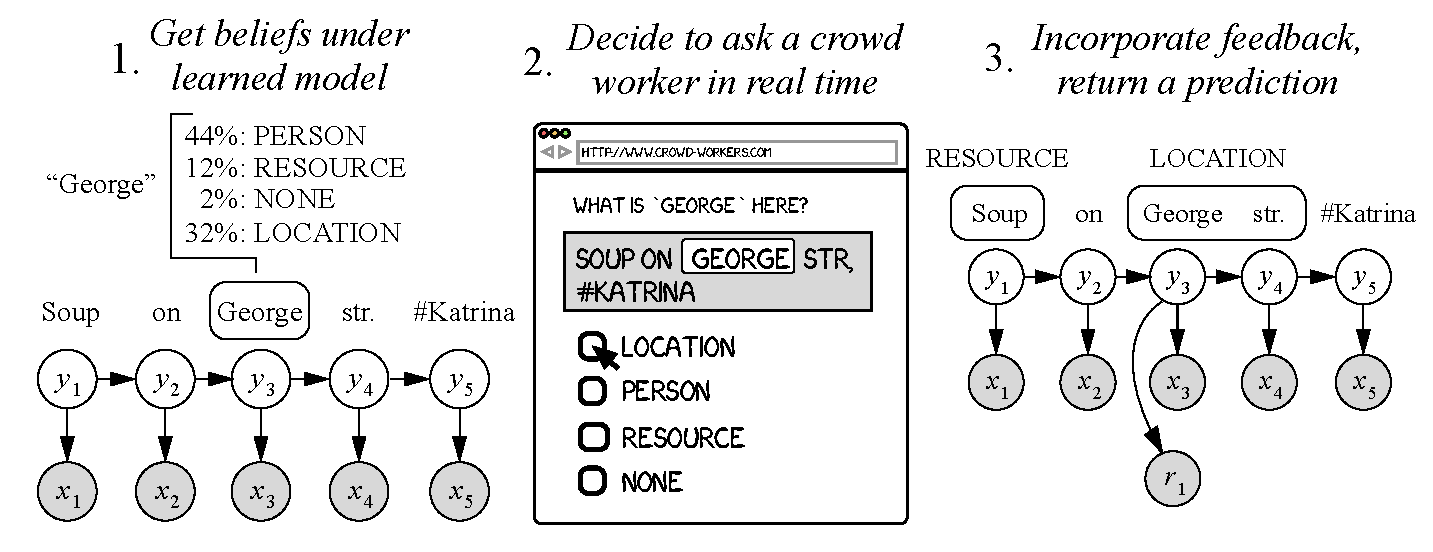
\includegraphics[width=1.0\textwidth]{figures/intro-banner.pdf}
  \end{centering}
  \caption{A figure showing an example of the Active Querying setting: Semantic slotfilling for Tweets during a disaster. We are interested in the tweet \textit{``Soup on George str.\ \#Katrina.''} The system first runs a pre-trained model, discovers that the token ``George'' is ambiguous, and then asks a human for a label. The human label is returned in a few seconds, incorporated into the model, and the model then decides it has enough information to turn in a classification.}
\label{fig:crf}
\end{figure}

\begin{figure}[t]
  \begin{centering}
  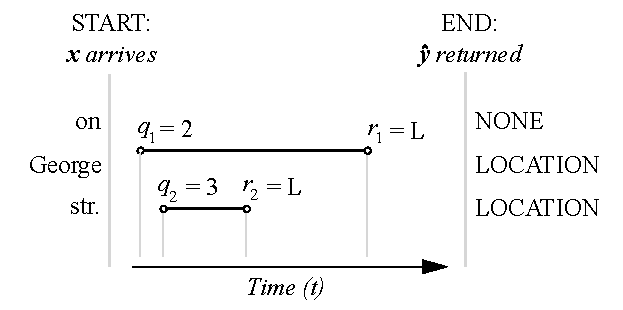
\includegraphics[width=1.0\textwidth]{figures/piano-roll.pdf}
  \end{centering}
  \caption{}
\label{fig:piano-roll}
\end{figure}

Let us make our problem setting concrete with an example, depicted in \figureref{piano-roll}.
We receive an input ``Soup on George str \#Katrina'' ($\bx$) and must produce an output ($\byt$) that labels words with the tags \scper{}, \scloc{}, \scres{} or \scnone{}.
Initially, our model is uncertain about both ``George'' and ``str''.
We first query the crowd for a label on ``George'' ($q_1$) and then for a label on ``str'' ($q_2$). 
After some time, the crowd responds with the label \scloc{} on both ``George'' ($r_1$) and ``str'' ($r_2$).
At this point, the model is confident in its labeling, and we can turn in its prediction $\byt$.
By querying the crowd, our model is able to produce a more accurate output, but we incur a cost for the queries as well as a time delay, $t$.

We would like to reason about the trade offs between accuracy, time and cost in a Bayesian decision theoretic framework.
Suppose the true output for the input $\bx$ was $\by$.
Let the (unobserved) reward at each step be the accuracy, $1 - \ell(\by, \byt)$.
Our utility is then 
\begin{align*}
u &= 1 - \ell(\by, \byt) + C(Q, t),
\end{align*}
where $Q = (q_1, q_2)$ is the sequence of queries made on the example and $t$ is the time so far.

We do not get to observe the labels $\by$, so instead our objective is to maximize our expected utility under our model:
\begin{align*}
  u &= \E_{\by \sim \p}[1 - \ell(\by, \byt) + C(Q, t)].
\end{align*}

%We receive a stream of inputs $\bx\oft1, \bx\oft2, \ldots, \bx\oft N$ with corresponding {\em unobserved\/} true output $\by\oft1, \by\oft2, \ldots, \by\oft N$ that we would like to predict.
%For each input $\bx$, we may query the crowd several times. Let $Q = \{q_1, \ldots, q_m\}$ be the set of queries.
%Finally, we observe responses $R = \{r_1, \ldots r_m\}$ to our queries after some time $t$.
%Using the information from these queries, our model makes the prediction, $\byt\oft{t}$.
%Our goal is to maximize the accuracy, trading off cost and latency as specified by a given objective function.
%
%More formally, suppose the output $\by\oft{t}$ has $n$ parts: $\by\oft{t} = y\oft{t}_1, \dots, y\oft{t}_n$.
%Let $q\oft{t} \in \{1, \ldots, n\}$ be a request for the label $y\oft{t}_q$,
%let $Q\oft{t} = (q\oft{t}_1, \dots, q\oft{t}_m)$ be a sequence of queries made on the $t$-th input and
%let $\tau\oft{t}$ be the time taken to make the prediction $\byt\oft{t}$. 
%We would like to minimize the cumulative loss, 
%following objective:
%\begin{align}
%  \sL &= \sum_{t=1}^T \ell_{\rmclass}(\by\oft{t}, \byt\oft{t}) + C(Q\oft{t}, \tau\oft{t}), \label{eqn:objective}
%\end{align}
%where $\ell_{\rmclass}$ is a given misclassification loss function, e.g.\ the Hamming loss, and $C$ is a given cost function.
%\ac{Concern: by using the cumulative loss, is there an expectation that we will ``model'' input and optimize for the future?}
%
%We now describe our choice of models for prediction, human error and latencies and return to optimizing \equationref{objective} in \sectionref{async}.
%
